% Assignment 3 research report. Build from assignment3/report/ with:
%   tectonic -X compile main.tex
% Tables and figures are read from ../analysis (generated by analysis/analyze.py).
\documentclass[11pt,a4paper]{article}

\usepackage[T1]{fontenc}
\usepackage{lmodern}
\usepackage{microtype}
\usepackage[margin=2.4cm]{geometry}
\usepackage{amsmath}
\usepackage{booktabs}
\usepackage{array}
\usepackage{graphicx}
\usepackage{xcolor}
\usepackage{listings}
\usepackage[font=small,labelfont=bf]{caption}
\usepackage{subcaption}
\usepackage{enumitem}
\usepackage[hidelinks]{hyperref}
\usepackage{url}
\usepackage[section]{placeins} % floats stay within their section

\graphicspath{{../analysis/figures/}}
\newcommand{\tabledir}{../analysis/tables}
\newcommand{\repourl}{\url{https://github.com/Xami650/Individual-Assignments-Big-Data-ULPGC}}
\newcommand{\session}{\texttt{20261104-030623}}

\lstset{
  basicstyle=\ttfamily\footnotesize,
  columns=fullflexible,
  keepspaces=true,
  frame=single,
  framesep=3pt,
  rulecolor=\color{black!30},
  aboveskip=4pt,
  belowskip=2pt,
  showstringspaces=false,
}

\setlist{itemsep=2pt,topsep=4pt}
% let lines with long unbreakable \texttt names stretch instead of overflowing
\setlength{\emergencystretch}{3em}

\title{\textbf{Assignment 3: Parallel Matrix Multiplication in Java}\\[4pt]
\large Thread Scaling of a Row-Parallel i-k-j Kernel on a 4+6-Core Apple M4,\\
with SIMD Vectorisation}
\author{Máximo Prosperi Reynoso\\[2pt]
\small BIG DATA, GCID, ULPGC\\
\small Individual Assignment 3, 2026--2027\\[2pt]
\small \repourl}
\date{4 November 2026}

\begin{document}
\maketitle

\begin{abstract}
\noindent
This study asks how the number of worker threads changes the performance of a
shared-memory matrix multiplication in Java, and when parallel execution
helps. The validated i-k-j kernel of Assignment~2 is the sequential baseline.
The parallel version computes the rows of $C$ with the same loop on a fixed
pool of $p=1$ to 20 worker threads, with rows claimed one at a time (dynamic)
or assigned in contiguous bands (static), for $n=64$ to 4096 on an Apple M4
with 4 performance (P) and 6 efficiency (E) cores. All 167 configurations gave
bitwise-identical results. Parallel execution helped from $n=128$ on. With the
4 P cores the speedup was 2.3 to 2.8, and with all 10 cores it was 3.0 to 4.3
for $n\ge256$, an efficiency of 0.30 to 0.43. At $n=64$ a multiplication lasts
30\,$\mu$s: the best speedup was 1.15, and with one thread the parallel code was
24\% slower than the sequential one. Per-process counters, including the CPU
time spent on P cores, explain why 10 threads were not 10 times faster. macOS
ran four threads on the P cores and the others on E cores, which retired 0.46
to 0.64 times the instructions per second of a P core. The clock fell from
4.0\,GHz with one busy core to 3.0 to 3.8\,GHz on the P cores and 2.8 to
2.9\,GHz on the E cores. Contention for the shared caches and memory raised the cycles per
multiply-add by 11 to 50\% with four threads. At $n=4096$, from $p=4$ on, the
kernel requested the matrix $B$ at about the 120\,GB/s memory bandwidth of the
chip, and the speedup stayed between 2.4 and 3.6. Oversubscription (12 to 20
threads) cost at most 5\% and gained clearly only at $n=1024$. Against the
hypothesis, static bands were up to 32\% faster than dynamic rows at $n=256$
and 1024. The most likely cause is that adjacent rows, computed at the same
time by different threads, share cache lines. The JIT's SIMD vectorisation made
the kernel 1.16 to 1.51 times faster with 40 to 49\% fewer instructions, and
it gained less with more threads. Peak memory grew with $p$ only at small $n$,
from task objects allocated on every call. The conclusions hold for the tested
kernel and machine only.
\end{abstract}

% ===========================================================================
\section{Introduction and objective}

Assignment~2 made the sequential Java kernel 3 to 10 times faster by
reordering its loops to i-k-j, so that the innermost loop adds a multiple of a
row of $B$ to a row of $C$. That kernel still used one core, while the machine
of these studies has ten: four performance (P) cores and six efficiency (E)
cores. This study keeps the validated i-k-j kernel, computes the rows of $C$ on
several threads, and asks how the number of threads changes its performance.

\paragraph{Research question.} \emph{How does the number of worker threads
(1 to 20) affect the runtime, speedup, efficiency and memory of a row-parallel
version of the validated i-k-j matrix multiplication in Java, for $n=64$ to
4096 on a 10-core Apple M4, and when does parallel execution help?} The factors
are the thread count $p$ and the matrix size $n$, with the way rows are
assigned to threads (the schedule) as a secondary factor. The outcomes are the
time per multiplication, the speedup $S(p)=T_{seq}(n)/T_p(n)$, the efficiency
$E(p)=S(p)/p$, the overhead of the parallel code with one thread, the peak
memory of the process, and process counters that explain the times: CPU time,
the share of it spent on E cores, instructions and cycles. $T_{seq}$ is the
time of the sequential baseline and $T_p$ the time of the parallel method with
$p$ threads on the same inputs; both are medians. Thread counts above 10, the
number of logical processors, are \emph{oversubscribed}.

\paragraph{Vectorisation (optional extension).} \emph{How much does the
JIT's automatic SIMD vectorisation contribute at a fixed thread count, and
does its effect change with the number of threads?} The same code is run with
the vectoriser of the JIT compiler switched on (the default) and off.

\paragraph{Hypotheses.} The hypotheses below were fixed in the protocol file
(\texttt{config/bench.json}) before the reported session. They are predictions,
and Section~\ref{sec:discussion} tests them against the results.
\begin{itemize}
  \item[H1] The parallel method is bitwise identical to the sequential one for
  every thread count and schedule, with or without vectorisation.
  \item[H2] With one thread, the parallel method pays a fixed cost per call for
  handing the work to a pool thread: above 10\% at $n=64$, below 1\% from
  $n=512$.
  \item[H3] For $n\le128$ a multiplication is too short to amortise waking and
  joining $p$ threads: the speedup stays below 2 and can fall below 1.
  \item[H4] The gain per added thread is largest up to $p=4$, the number of P
  cores; threads beyond 4 run partly on E cores and add less, so $S(10)$ is well
  below 10. With a static assignment of rows the slowest core sets the time, so
  the static schedule is slower than the dynamic one for $4<p\le10$.
  \item[H5] The kernel reads all of $B$ for every row of $C$, so several cores
  compete for the shared cache and memory bandwidth: the cycles per
  multiply-add, summed over all cores, rise with $p$, more so for $n\ge2048$,
  where $B$ no longer fits in the L2 cache. No superlinear speedup is expected.
  \item[H6] Oversubscription gives no further speedup and, with the dynamic
  schedule, costs little (within 5\% of $p=10$).
  \item[H7] Peak memory does not depend on $p$ beyond a few MiB.
  \item[H8] Without vectorisation the compiled inner loop is scalar, the
  instructions per multiply-add roughly double, and the kernel slows down most
  where it is limited by execution ($p=1$, $n\le1024$) and least where it is
  limited by memory traffic ($p=10$, $n=2048$).
\end{itemize}

% ===========================================================================
\section{Background and references}

\paragraph{Speedup and its limits.} If a fraction $f$ of a computation cannot
be parallelised, $p$ processors give at most $S(p)=1/((1-f)+f/p)$, Amdahl's
bound~\cite{amdahl1967}. In a parallel matrix multiplication with fixed work
per row, the serial part is the time to start and join the threads, and the
idle time at the end of a call when the rows run out unevenly. On a chip whose
cores differ in speed, $p$ threads do not add up to $p$ cores of work either:
Hill and Marty extend Amdahl's model to such asymmetric chips~\cite{hill2008}.
A kernel can also be limited by memory traffic rather than by arithmetic. The
roofline model bounds the attainable rate by the memory bandwidth times the
operational intensity, the floating-point operations per byte moved from
memory~\cite{williams2009}. When several cores share a cache or a memory
channel, the bandwidth per core falls as cores are added. The clock rate also
varies: chips run their cores faster when few are active and slow them down as
power and temperature rise~\cite{hennessy2019}.

\paragraph{Assigning rows to threads.} In the i-k-j order, the rows of $C$ are
independent: row $i$ depends on row $i$ of $A$ and on all of $B$, which are
only read. The rows can be split among threads in two classic ways, named after
OpenMP's \texttt{schedule} clause~\cite{openmp52}. A \emph{static} schedule
fixes the assignment in advance, for example one contiguous band of $n/p$ rows
per thread, and costs nothing at run time. A \emph{dynamic} schedule lets each
thread claim the next unclaimed chunk of rows when it becomes free, which costs
a shared counter but adapts to threads that run at different speeds. On Apple
silicon, Apple's tuning guide warns that ``if you use a static distribution,
threads running on higher efficiency cores will finish much sooner than threads
running on lower efficiency cores''~\cite{appletuning}.

\paragraph{Java threads and shared data.} The Java memory model defines when a
write by one thread is visible to a read by another: only if the write
\emph{happens-before} the read (JLS \S17.4.5~\cite{jls25}). The classes of
\texttt{java.util.concurrent} extend this to their operations: actions before
the submission of a task to an \texttt{ExecutorService} happen-before the task
runs, and ``actions taken by the asynchronous computation represented by a
\texttt{Future} happen-before actions subsequent to the retrieval of the result
via \texttt{Future.get()} in another thread''~\cite{juc25}. A fixed thread pool
keeps its threads alive between calls, so a call pays for waking them, not for
creating them~\cite{goetz2006}.

\paragraph{Cores and scheduling on macOS.} The Apple M4 has four P cores,
which share a 16\,MiB L2 cache, and six E cores, which share a 4\,MiB L2 cache.
macOS decides on which core type a thread runs; an application influences this
only through the quality-of-service (QoS) class of its work, and background
work tends to run on the E cores~\cite{appletuning}. There is no way to bind a
thread to a core: on the machine of this study, the affinity interface of the
kernel (\texttt{thread\_policy\_set} with \texttt{THREAD\_AFFINITY\_POLICY})
returns \texttt{KERN\_NOT\_SUPPORTED}. macOS does account the CPU time,
instructions and cycles of a process separately for the P cores
(\texttt{struct rusage\_info\_v6}, returned by
\texttt{proc\_pid\_rusage}~\cite{macsdk}), which this study uses to see where
its threads ran.

\paragraph{SIMD vectorisation.} HotSpot's optimising JIT compiler (C2) packs
independent iterations of simple loops into SIMD instructions with its
SuperWord pass, after the superword-level parallelism method of Larsen and
Amarasinghe~\cite{larsen2000}. On the M4 the vectors are 128-bit NEON registers,
which hold two doubles. The pass is on by default and is switched off with
\texttt{-XX:-UseSuperWord}. Java forbids contracting $a\cdot b+c$ into a fused
multiply-add~\cite{jep306}, so vector and scalar code perform the same rounded
operations. Assignment~2 inferred vectorisation from instruction counts only.

\paragraph{Measuring Java code.} The JIT compiles a method while it runs, so
the first executions run different code from the steady state, and benchmarks
must discard warm-up iterations~\cite{georges2007}. Assignment~2 found that a
single long call could stay in on-stack-replacement code unless the method was
first compiled on small inputs, and added a pre-warm for this reason.

% ===========================================================================
\section{Methodology}
\label{sec:method}

\subsection{Implementations}

All code is in \texttt{src/main/java/org/ulpgc/bd/matmul/} and was written for
this study, except the baseline, which is copied unchanged from Assignment~2.
No library is used in any measured method. Both methods compute in IEEE-754
double precision on the same \texttt{double[][]} storage (an array of row
arrays) and the same inputs, and both perform the same i-k-j loop for every row
(Fig.~\ref{fig:kernels}).
\begin{itemize}
  \item \textbf{ikj} (sequential baseline, \texttt{DenseMatMul.ikj}): the i-k-j
  kernel of Assignment~2 (tag \texttt{assignment2-v1.0}), validated there
  against NumPy and bitwise against the Assignment~1 baseline. It runs on the
  main thread and no thread pool exists.
  \item \textbf{par\_ikj} (parallel, \texttt{ParallelMatMul.ikj}): the rows of
  $C$ are distributed among $p$ worker threads, and each row is computed by
  \texttt{ikjRow}, the loop body of ikj for one $i$. The workers belong to a
  \texttt{ThreadPoolExecutor} with exactly $p$ threads, created and started
  before any timing. A call builds $p$ tasks, hands them to the pool with
  \texttt{invokeAll} and waits; the calling thread never computes a row, so $p$
  counts the threads that compute. Two schedules assign the rows:
  \begin{itemize}
    \item \emph{dynamic} (the main configuration): each worker claims the next
    unclaimed row from a shared \texttt{AtomicInteger}, one row at a time,
    until none are left;
    \item \emph{static}: worker $t$ computes the contiguous band of rows from
    $\lfloor tn/p\rfloor$ to $\lfloor(t+1)n/p\rfloor-1$.
  \end{itemize}
\end{itemize}
\textbf{Shared data.} $A$ and $B$ are only read, and each row of $C$ is written
by exactly one task. The inputs exist before the tasks are submitted, and
\texttt{invokeAll} returns only after every task has completed; the
happens-before guarantees of the executor and of \texttt{Future.get()}
(Section~2) make every write of a worker visible to the caller. Rows are
separate arrays, so two threads can touch the same 128-byte cache line only at
the boundary between two row arrays. Every entry $C_{ij}$ receives the same
operations in the same order as in ikj, so the results should be bitwise
identical (H1).

\begin{figure}[tbp]
\centering
\begin{subfigure}[t]{0.48\linewidth}
\begin{lstlisting}[language=Java]
// row i of C (ikjRow; ikj loops it over i)
double[] ai = a[i], ci = c[i];
Arrays.fill(ci, 0.0);
for (int k = 0; k < n; k++) {
  double aik = ai[k]; double[] bk = b[k];
  for (int j = 0; j < n; j++)
    ci[j] += aik * bk[j];
}
\end{lstlisting}
\end{subfigure}\hfill
\begin{subfigure}[t]{0.48\linewidth}
\begin{lstlisting}[language=Java]
// par_ikj: one task per worker thread
// dynamic
for (int i = next.getAndIncrement(); i < n;
     i = next.getAndIncrement())
  ikjRow(a, b, c, n, i);
// static, worker t of p
for (int i = t*n/p; i < (t+1)*n/p; i++)
  ikjRow(a, b, c, n, i);
// caller: pool.invokeAll(tasks), then get()
\end{lstlisting}
\end{subfigure}
\caption{The measured code (abbreviated). \texttt{next} is a fresh
\texttt{AtomicInteger} per call; the bounds of the static bands use 64-bit
arithmetic.}
\label{fig:kernels}
\end{figure}

\subsection{Inputs}

The inputs are those of Assignments~1 and~2, generated by the same unchanged
code: for each $n$, $A$ and then $B$ are drawn uniformly on $[-1,1)$ from
NumPy's PCG64 generator~\cite{harris2020} seeded with
\texttt{SeedSequence([2026, n])}, and stored as raw little-endian float64. All 24
files used here (12 sizes) have the same SHA-256 digests as the Assignment~2
files, which are tracked in \texttt{data/checksums.sha256}.

\subsection{Experiments}

Table~\ref{tab:experiments} lists the three experiments of the reported
session, 167 configurations in all, each run in its own JVM process. Thread
counts from 1 to 10 locate the changes at $p=4$ (the P cores) and $p=10$ (all
logical processors). Counts of 12, 16 and 20 are oversubscribed. The sizes
bracket the caches. $B$ takes 32\,KiB at $n=64$ and 2\,MiB at $n=512$, which
fits both L2 caches. At 1024 it takes 8\,MiB, which fits only the 16\,MiB L2
of the P cores, and at 2048 and 4096 it takes 32 and 128\,MiB, which fit
neither. In every size block, the sequential ikj and the parallel method with
10 threads also run at the start and at the end as drift controls
(Section~\ref{sec:protocol}).

\begin{table}[tbp]
\centering
\caption{Experiments of the reported session (167 configurations). The
SuperWord-on counterparts of V\_simd are the P\_threads configurations with the
same method, $n$ and $p$.}
\label{tab:experiments}
\small
\begin{tabular}{@{}l>{\raggedright\arraybackslash}p{0.3\linewidth}>{\raggedright\arraybackslash}p{0.36\linewidth}r@{}}
\toprule
Experiment & Methods & Sizes and threads & Configs \\
\midrule
P\_threads & ikj; par\_ikj, dynamic & $n=64$, 128, 256, 512, 1024, 2048, 4096; $p=1$ to 10, 12, 16, 20 & 119\textsuperscript{a} \\
P\_schedule & par\_ikj, static & $n=256$, 1024, 2048; same $p$ & 39 \\
V\_simd & \texttt{-XX:-UseSuperWord}: ikj; par\_ikj, dynamic, $p=4$ and 10 & $n=512$, 1024, 2048 & 9 \\
\bottomrule
\end{tabular}
\par\smallskip{\footnotesize\raggedright \textsuperscript{a} 91 par\_ikj
configurations and 28 drift controls (ikj and par\_ikj with $p=10$, first and
last in each of the 7 size blocks).\par}
\end{table}

\subsection{Execution environment}

Table~\ref{tab:env} lists the machine and the software. These settings were
the same for every run.

\begin{table}[tbp]
\centering
\caption{Execution environment and fixed settings of the reported session
(\session, recorded in \texttt{env.txt} before and after the session).}
\label{tab:env}
\small
\begin{tabular}{@{}lp{0.74\linewidth}@{}}
\toprule
Machine & MacBook Air 15-inch, M4, 2025 (Mac16,13), fanless; 24\,GiB RAM with
120\,GB/s memory bandwidth~\cite{applem4}; AC power, Low Power Mode off \\
CPU & Apple M4: 4 P cores (L1d 128\,KiB each, 16\,MiB L2 shared) and 6 E cores
(L1d 64\,KiB each, 4\,MiB L2 shared); 10 physical cores and 10 logical
processors (no SMT); 128\,B cache lines; 16\,KiB pages \\
Affinity & none: \texttt{thread\_policy\_set} with
\texttt{THREAD\_AFFINITY\_POLICY} returns \texttt{KERN\_NOT\_SUPPORTED} (46);
the scheduler places the threads, and the P-core share of CPU time is measured \\
OS & macOS 26.6.2 (build 25G83), Darwin 25.6.0 \\
Java & OpenJDK 25.0.1 (build 25.0.1+8-27, HotSpot 64-bit Server VM), Maven
3.9.12; \texttt{java -Xmx8g}; defaults otherwise: G1 collector (4\,MiB regions,
9 parallel and 2 concurrent GC threads), tiered compilation with 4 compiler
threads, SuperWord on, 16-byte maximum vector size, 2\,MiB thread stacks \\
Threads & with ikj the process has 6 Java threads (21 operating-system threads,
including the JIT and GC threads); par\_ikj adds its $p$ workers (16 and 31 at
$p=10$, 26 and 49 at $p=20$) \\
Python & CPython 3.13.9 (Anaconda build) with NumPy 2.3.5, pandas 2.3.3,
matplotlib 3.10.6 and psutil 7.0.0, only for inputs, checks, the harness and
the analysis \\
Source & commit \texttt{1736461}; only the drafts of the report, the README
and the analysis script were uncommitted \\
Conditions & 43.1\,min starting at 03:06 on 4~November 2026, with the desktop
applications and a container virtual machine closed; no thermal or
performance warning before or after; 1-minute load average 1.27 at the start
(just after the build); other processes used a median of 0.06 cores during the
runs \\
\bottomrule
\end{tabular}
\end{table}

\subsection{Process counters and resource metrics}

Around every sample, the driver reads the counters of its own process through
the Java foreign function interface~\cite{jep454}:
\texttt{proc\_pid\_rusage} with \texttt{RUSAGE\_INFO\_V6} gives the CPU time
(user plus system), the part of it on P cores, the instructions and the cycles,
each in total and on P cores; \texttt{proc\_pidinfo} gives the context switches
and the number of threads of the process~\cite{macsdk}. All are sums over the
threads of the process. From the differences over the measured samples the
analysis derives, per configuration: the busy cores $U$ (CPU time divided by
elapsed time), the share of CPU time on E cores, the mean clock rate of the
busy cores $f$ (cycles divided by CPU time), and the cycles and instructions
per multiply-add. Ratios of sums make the identity $T=C/(fU)$ exact for the mean
time per multiplication $T$ and the cycles per multiplication $C$, so the
speedup of the means splits into three factors,
\[
\bar S=\frac{C_{seq}}{C_p}\cdot\frac{f_p}{f_{seq}}\cdot\frac{U_p}{U_{seq}},
\]
extra cycles (contention), clock rate (frequency and core type) and idle
threads. The driver also records the garbage collections, the JIT compilation
time and the bytes allocated on the Java heap during the measured samples, the
number of Java and operating-system threads, and the CPU time of the process
per QoS class. Around every process, the harness reads the system-wide CPU time
(\texttt{psutil}) and subtracts the process's own CPU time, which gives the CPU
time used by other processes during the run.

\textbf{Memory} is measured as in Assignments~1 and~2: the peak resident set
size (RSS) and the peak memory footprint of the whole process, from
\texttt{/usr/bin/time -l}, next to the element storage of the three matrices,
$24n^2$ bytes.

\subsection{Correctness checks}
\label{sec:correctness}

The Java code has 32 JUnit~5 tests. They cover hand-computed $2\times2$ and
$3\times3$ products, identity and zero matrices, an exact BigDecimal reference,
the overwriting of a reused output, and par\_ikj bitwise against ikj for
$n\in\{1,2,3,7,33,64,65,100\}$, $p\in\{1,2,3,4,7,10,16,20\}$ (so also $p>n$)
and both schedules. Further tests make 200 repeated calls on one pool, to
expose races between calls, and check the static bands, the propagation of an
exception thrown in a worker, the rejection of $p<1$, the process counters, the
file format and the driver's output contract.

Before benchmarking, \texttt{scripts/verify.py} ran 15 configurations through
their normal command line: ikj; par\_ikj with $p\in\{1,2,3,4,10,16\}$ and both
schedules; and ikj and par\_ikj ($p=4$) with SuperWord off. The cases are those
of Assignments~1 and~2: $n\in\{1,2,3,10,64,100,256\}$ with random inputs
(reference \texttt{numpy.matmul}), $AI$ (exact answer $A$) and $A\cdot0$ (exact
answer $0$). A result passes if $|C_{ij}-R_{ij}|\le 2\gamma_n(|A||B|)_{ij}$ for
every entry, with $\gamma_n=nu/(1-nu)$ and $u=2^{-53}$. This is the tolerance of
Assignment~1: it bounds the difference between two results computed in any
summation order~\cite{higham2002}. In addition, all configurations of a case
must agree bit for bit (H1). During the benchmark, every sample prints the sum
of the entries of $C$. This consumes the result, and it is compared across all
configurations of each $n$.

\subsection{Measurement protocol}
\label{sec:protocol}

The protocol is that of Assignment~2, with drift controls and cool-down pauses
added for the parallel runs.

\paragraph{Timer boundary.} Only the multiplication is timed, with
\texttt{System.nanoTime()}. For ikj this is the kernel call, including the
clearing of each row of $C$. For par\_ikj it is the whole
\texttt{ParallelMatMul.ikj} call: building the $p$ tasks, handing them to the
workers, which are already running, the computation, and the wait until every
task has finished. Creating the pool and starting its threads, loading the
inputs, starting the JVM and the pre-warm are outside the timed region. The
time of par\_ikj with one thread therefore includes the cost of handing the work
to another thread, which is the overhead the assignment asks for.

\paragraph{Pre-warm, warm-up and samples.} Each configuration runs in one fresh
JVM. The JVM creates its pool and then runs the method for 1\,s on small random
inputs ($n=\min(N,256)$) with the same pool, so that the JIT compiles the kernel
with a complete profile. Warm-up then continues until at least one sample and
1\,s of warm-up work have run. Each sample times $k$ back-to-back
multiplications, with $k=\max(1,\lceil 0.1\,\text{s}/t\rceil)$ and $t$ the time
per multiplication of the latest warm-up. Five measured samples follow. The
summaries report the median and the interquartile range (IQR) of the time per
multiplication over these five samples. Warm-up samples are kept in the raw
data and excluded from every summary.

\paragraph{Speedup.} $S(p)$ is the median time of the first ikj run of the same
size block divided by the median time of the configuration, and
$E(p)=S(p)/p$. Its interval, shown as error bars, is
$[Q_1^{seq}/Q_3^{p},\,Q_3^{seq}/Q_1^{p}]$.

\paragraph{Run order, drift controls and cool-down.} The session runs one block
per size, in ascending $n$. Each block starts with ikj and par\_ikj (dynamic,
$p=10$) and ends with the same two in reverse order. The other configurations
of that size run in between, in the order given by
\texttt{random.Random(2026\,+\,n).shuffle} over the declared list, so that the
thread count is not confounded with the time within the block. The last/first
ratios of the two controls measure the drift of the machine over the block, for
one core and for all cores. After each process the harness pauses for as long
as the process ran, at least 5\,s and at most 90\,s.

\paragraph{Pilot.} A pilot session, not part of the reported data ($n=2048$ and
4096, two samples per configuration, 2\,s pauses), fixed the session length. It
also showed thermal throttling. In the multi-threaded runs at $n=4096$, the mean
clock of the busy cores (cycles per CPU second) fell from about 3.1\,GHz at the
start of the block to about 2.0\,GHz at its end, while single-thread runs stayed
at 4.0\,GHz; the MacBook Air has no fan. A drift control with one thread cannot
see this. The cool-down pauses and the drift control with all cores were
therefore added and declared in the protocol before the reported session.

\paragraph{Budgets.} Each process had 60\,s to load its inputs, create the pool
and pre-warm, and then at most 120\,s for every sample. The heap was limited to
8\,GiB (\texttt{-Xmx8g}) and the session to 90\,min. A failure would have been
recorded as a result; none occurred.

\paragraph{Background load.} Around every process, the harness reads the
system-wide busy CPU time (\texttt{psutil}) and subtracts the CPU time of the
process, which gives the CPU time used by other processes during the run. In
the reported session, \texttt{/usr/bin/time} printed its times with a decimal
comma, because the shell ran under a Spanish locale, and the harness did not
parse them. The analysis therefore takes the process's CPU time from the CPU
times per QoS class that the driver reads from \texttt{proc\_pid\_rusage} at
exit, which cover the whole process. In the pilot and a smoke session, which
recorded both, the two agreed within 0.02\,s per process. The parser was fixed
after the session.

\subsection{Vectorisation evidence}

Two kinds of evidence show what the vectoriser does. The first is the machine
code. \texttt{scripts/simd\_evidence.py} runs the driver once with SuperWord on
and once with it off, for ikj and for par\_ikj ($p=4$, dynamic, $n=512$), with
HotSpot's diagnostic \texttt{-XX:CompileCommand=print}. These flags are used
only in this separate run, never in a timed one. Without the \texttt{hsdis}
disassembler plugin, HotSpot prints the compiled code as hexadecimal
instruction words. The script turns them back into instructions with
\texttt{clang} (as \texttt{.inst} directives) and \texttt{objdump}. In the
final C2-compiled code of each kernel method, it then counts the two-lane
vector (\texttt{fmul.2d}, \texttt{fadd.2d}) and the scalar double-precision
multiplies and adds, the fused multiply-adds, and the 128-bit (\texttt{q}
register) loads and stores. The files were regenerated after the session with
the session's JDK. The counts equal those of the files produced on the day of
the pilot, when the default JDK was OpenJDK 25.0.2. The second kind of evidence is the counters: the
instructions and cycles per multiply-add of the V\_simd configurations and of
their SuperWord-on counterparts.

% ===========================================================================
\section{Results}
\label{sec:results}

\subsection{The session and its controls}
\label{sec:session}

The session ran 167 configurations in 43.1\,min, and all completed with five
measured samples. The relative IQR was 0.42\% in the median configuration and
at most 10.7\% (static, $p=12$, $n=2048$). It exceeded 2\% in 20
configurations: 14 at $n\ge2048$ and 6 static runs at $n=256$ and 1024. Other
processes used a median of 0.06 cores during the runs (90th percentile 0.18,
maximum 1.29 in a single run). One garbage collection, shorter than 1\,ms, fell
into a measured sample (par\_ikj, $p=4$, $n=64$). The JIT compiler threads were
still active during the measured samples of every configuration, for 2 to
25\,ms of compilation time (median 4\,ms). That is at most about 5\% of the
measured time, and it ran on a compiler thread, not in the timed kernel.

The drift controls (Table~\ref{tab:overhead}, last two columns) stayed within
$\pm1.2\%$ for ikj except at $n=128$. There, the last run was 7.4\% faster than
the first, with the same instructions per multiply-add and the same 4.04\,GHz
clock but fewer cycles (0.540 against 0.583 per multiply-add). The difference
lies between two JVMs running the same code, and every speedup at $n=128$
depends on the choice of baseline run by up to 7.4\%. For $p=10$, the ratio was
0.996 to 1.033, except at $n=2048$ (0.875). The first $p=10$ run at that size
took 380\,ms, against 330 and 332\,ms for the shuffled and the last run. It used
11\% more cycles per multiply-add for the same instructions while other
processes used 0.40 cores; the speedups use the shuffled run. At $n=4096$ the
last $p=10$ run, at the end of a block of about 20\,min, ran its cores at
2.59\,GHz instead of 3.03\,GHz, a sign of thermal throttling. It still took only
2.5\% longer, because its cycles per multiply-add fell by 12\%.

\subsection{Correctness}

All 32 unit tests passed; they were run again with the session's JDK.
\texttt{verify.py} checked 315 (case, configuration) results. All were within
the tolerance (largest error 0.13 of the bound), and in every case all 15
configurations were bitwise identical. In the benchmark session, the checksums
of every configuration agreed exactly for each $n$ (167 configurations, 835
measured samples).

\subsection{Time, speedup and efficiency}

Table~\ref{tab:time} gives the median time per multiplication, and
Table~\ref{tab:speedup} the speedups and efficiencies. Fig.~\ref{fig:speedup}
plots them against $p$, and Fig.~\ref{fig:size} against $n$. With four threads,
the number of P cores, the speedup was 2.3 to 2.8 for every $n\ge128$. Threads
beyond four raised it more slowly, to 3.0 to 4.3 at $p=10$ for $n\ge256$. The
efficiency fell with every added thread, from 0.58 to 0.69 at $p=4$ to 0.30 to
0.43 at $p=10$ ($n\ge256$). The largest speedup with at most 10 threads was
4.27 ($n=1024$); with 16 threads at the same size it was 4.86. Against $n$, the
speedup with 10 or more threads rose to its maximum at $n=1024$ and fell at
2048 and 4096. With four threads it stayed between 2.3 and 2.8 from $n=128$
on.

\begin{table}[tbp]
\centering
\caption{Median time per multiplication (ms) of ikj and of par\_ikj (dynamic)
for each $p$ and $n$. Last row: the largest relative IQR among the
configurations of the column.}
\label{tab:time}
\small
\input{\tabledir/tab_time.tex}
\end{table}

\begin{table}[tbp]
\centering
\caption{Speedup $S(p)$ and, in parentheses, efficiency $E(p)$ of par\_ikj
(dynamic) over the first ikj run of each size block.}
\label{tab:speedup}
\small
\input{\tabledir/tab_speedup.tex}
\end{table}

\begin{figure}[tbp]
\centering
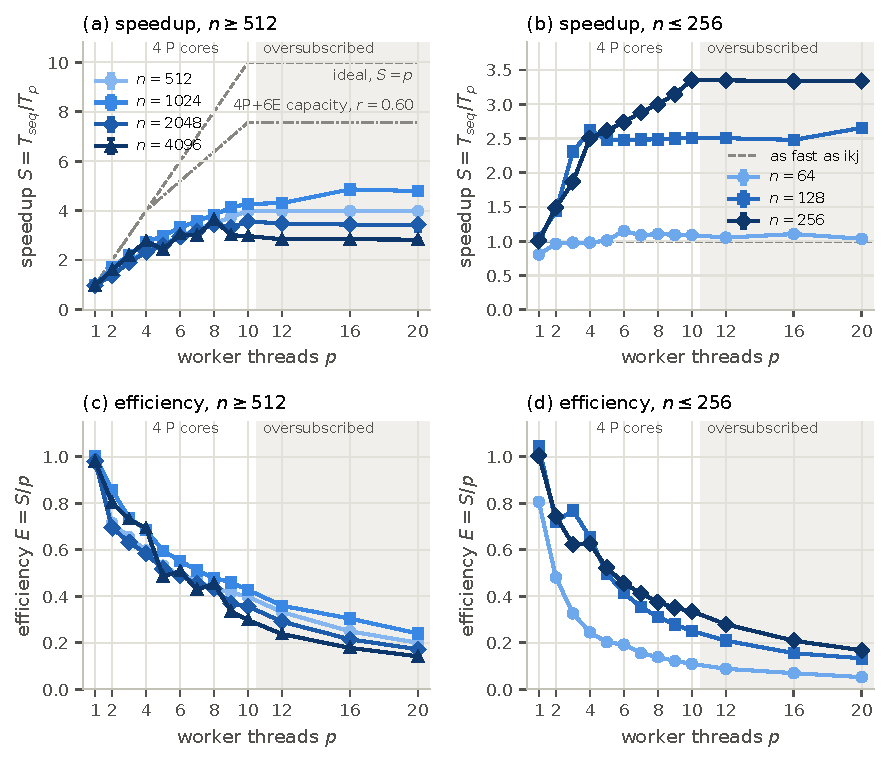
\includegraphics[width=\linewidth]{fig_speedup.pdf}
\caption{Speedup (top) and efficiency (bottom) of par\_ikj (dynamic) against
the number of worker threads, for $n\ge512$ (left) and $n\le256$ (right).
Error bars: $[Q_1^{seq}/Q_3^{p},Q_3^{seq}/Q_1^{p}]$. Dotted lines: $p=4$ (P
cores) and $p=10$ (logical processors); shaded: oversubscribed. The 4P+6E
capacity line, $\min(p,4)+r\,\mathrm{clip}(p-4,0,6)$, counts an E core as
$r=0.60$ P cores, the ratio of instructions per CPU second on E and P cores
measured at $p=10$, $n=512$. At $n=128$, $E(1)>1$ because the first ikj run,
the baseline, was 7.4\% slower than the last (Section~\ref{sec:session}).}
\label{fig:speedup}
\end{figure}

\begin{figure}[tbp]
\centering
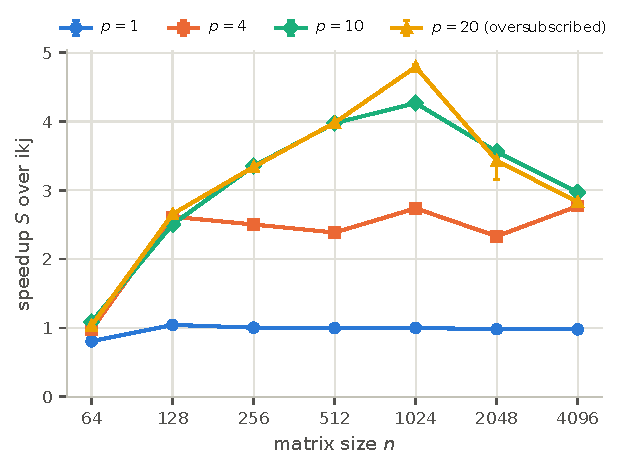
\includegraphics[width=0.68\linewidth]{fig_size.pdf}
\caption{Speedup over ikj against $n$ for $p=1$, 4, 10 and 20 (dynamic), with
the same interval bars as Fig.~\ref{fig:speedup}.}
\label{fig:size}
\end{figure}

At $n=64$ a sequential multiplication took 30.0\,$\mu$s. No thread count made
it more than 1.15 times faster (at $p=6$), and with one to four threads the
parallel method was slower than ikj ($S=0.81$ to 0.98). With 10 threads the
process kept only 2.9 cores busy on average, and it made 226\,000 context
switches per second, against about 2\,000 at $n\ge1024$. At $n=128$ (0.30\,ms)
the speedup reached 2.6 at $p=4$ and stayed between 2.5 and 2.7 for every larger
$p$. The busy cores levelled off at 4.2 to 4.5, and the E cores did 7 to 9\% of
the work.

\subsection{One thread: the cost of the hand-off}

With one thread, par\_ikj was 24.0\% slower than ikj at $n=64$, which is
7.2\,$\mu$s per call for handing the work to a worker and waiting for it
(Table~\ref{tab:overhead}). From $n=256$ to 1024 the difference was within
$\pm0.4\%$. At $n=128$ it was $-4.3\%$ against the first ikj run and $+3.4\%$
against the last, so it is smaller than the 7.4\% between the two baseline
runs. At $n=2048$ and 4096 the one-thread version was 1.9 and 2.1\% slower than
the first ikj run (2.1 and 0.8\% against the last). A cost of microseconds per
call cannot explain this. The counters show the same instructions per
multiply-add (within 0.02\%) at the same 4.04\,GHz, but 1.9 to 2.0\% more
cycles. The static schedule with one thread behaved the same way (+0.9\% at
$n=2048$).

\begin{table}[tbp]
\centering
\caption{One thread, the best thread count and the drift, per $n$. overhead:
median time of par\_ikj (dynamic, $p=1$) relative to ikj; static: the same for
the static schedule (P\_schedule sizes only); best $p$: the fastest par\_ikj
configuration (dynamic), with its $S$ and $E$; drift: median time of the last
over the first control run of the block, for ikj and for par\_ikj with $p=10$.}
\label{tab:overhead}
\small
\setlength{\tabcolsep}{4pt}
\input{\tabledir/tab_overhead.tex}
\end{table}

\subsection{Where the threads ran and what limited them}

Fig.~\ref{fig:cores} shows how the threads used the cores. For $n\ge256$, the
busy cores $U$ followed $p$ up to 10 (9.3 to 9.9 at $p=10$), so the workers
were rarely idle. The share of CPU time on E cores was at most 1\% up to $p=4$.
From there it followed $(p-4)/p$ closely: 20, 33, 43, 50, 55 and 60\% for
$p=5$ to 10 at $n=1024$.
macOS therefore kept four threads on the P cores and ran every further thread
on an E core. Beyond 10 threads nothing changed: the busy cores and the E-core
share stayed at their $p=10$ values. At $p=10$, an E core retired 0.46 to 0.64
times as many instructions per CPU second as a P core ($n\ge256$; 0.60 at
$n=512$, the $r$ of Fig.~\ref{fig:speedup}). The clock fell as threads were
added. With one busy thread the P cores ran at 4.04\,GHz, with four at 3.1 to
3.7\,GHz, and the E cores ran at 2.8 to 2.9\,GHz.

\begin{figure}[tbp]
\centering
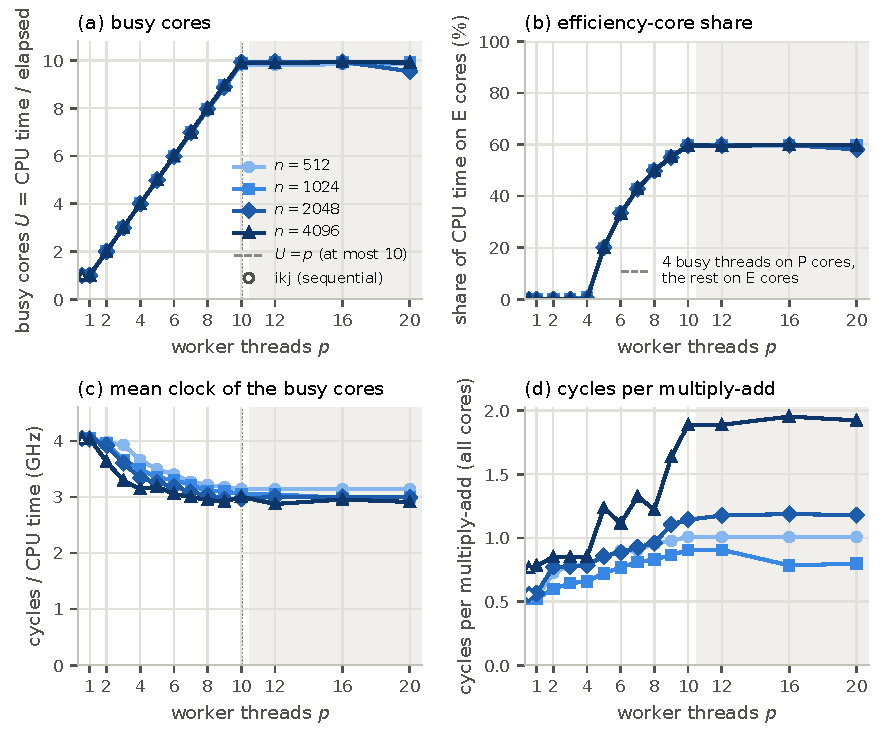
\includegraphics[width=\linewidth]{fig_cores.pdf}
\caption{Process counters of par\_ikj (dynamic) for $n\ge512$; hollow markers
at the left: ikj. (a) Busy cores, CPU time divided by elapsed time. (b) Share
of the CPU time on E cores, with the share expected if four busy threads run on
P cores and the others on E cores. (c) Mean clock of the busy cores, cycles
divided by CPU time. (d) Cycles per multiply-add, summed over all cores.}
\label{fig:cores}
\end{figure}

Table~\ref{tab:decomp} splits the mean speedup into its three factors. At
$p=10$ and $n=512$ to 4096, 9.8 to 9.9 busy cores gave speedups of only 3.0 to
4.3. Each multiplication needed 1.7 to 2.5 times the cycles of the sequential
run ($C_s/C_p=0.40$ to 0.58), and those cycles ran at 0.74 to 0.78 times the
sequential clock. Part of the extra cycles comes from the E cores, which need
more cycles per instruction. With four threads, however, all on P cores and with
the same instructions as ikj, the cycles per multiply-add were already 1.11 to
1.50 times the sequential ones ($n\ge256$). This is contention between the P
cores for their shared L2 cache and for memory.

\begin{table}[tbp]
\centering
\caption{Decomposition of the speedup of the means,
$\bar S=(C_s/C_p)(f_p/f_s)(U_p/U_s)$, for $n\ge512$ and selected $p$ (dynamic).
busy $U$: CPU time over elapsed time; E-core: share of the CPU time on E cores;
clock: cycles over CPU time; cycles and instructions per multiply-add are
summed over all cores; seq.: ikj.}
\label{tab:decomp}
\footnotesize
\setlength{\tabcolsep}{4pt}
\input{\tabledir/tab_decomp.tex}
\end{table}

Each multiply-add reads 8 bytes of $B$, so a multiplication that takes $T$
requests $B$ at $8n^3/T$ bytes per second from the memory hierarchy. At
$n=4096$, where $B$ occupies 128\,MiB, the sequential kernel requested
42\,GB/s. From $p=4$ on, the parallel kernel requested 103 to 154\,GB/s, and
120\,GB/s with 12, 16 and 20 threads. This is the memory bandwidth Apple
specifies for the M4~\cite{applem4}. If every byte of $B$ came from memory, the
speedup at $n=4096$ could not exceed $120/42\approx2.8$. The measured speedups
for $p\ge4$ were 2.4 to 3.6, and 2.8 for every oversubscribed $p$. At $n=2048$
($B=32$\,MiB), 10 threads requested 209\,GB/s, more than the memory can supply,
so part of $B$ came from the caches.

\subsection{Static against dynamic rows}

Contrary to H4, the static schedule was faster than the dynamic one at $n=256$
and 1024 for most thread counts above four (Fig.~\ref{fig:schedule},
Table~\ref{tab:schedule}). For $5<p\le10$ it was faster by 11 to 32\% at
$n=256$ and by 11 to 20\% at $n=1024$. At $p=5$ it was 1\% slower at $n=256$
and 18\% faster at $n=1024$. Only at $n=2048$ did static lose, by 8 to 16\% at
$p=6$, 7 and 10, while it was within 5\% at the other thread counts up to 10. The static runs did leave cores idle, as
H4 expected. At $p=10$ they kept 5.8 ($n=256$), 8.6 (1024) and 9.1 (2048) cores
busy, against 9.3 to 9.9 for the dynamic schedule. The E cores also did less of
the work: 24 to 38\% at $p=10$, not the 60\% of the rows that six of the ten
bands hold. Yet the static runs needed far fewer cycles per multiply-add for the
same instructions: 0.65 against 1.18 at $n=256$, and 0.69 against 0.90 at
$n=1024$ ($p=10$). The excess of the dynamic schedule shrank as $n$ grew: 0.53,
0.22 and $-0.09$ cycles per multiply-add at $n=256$, 1024 and 2048 ($p=10$). It
was present with four threads too (0.16 at $n=256$), when every thread ran on a
P core.

\begin{figure}[tbp]
\centering
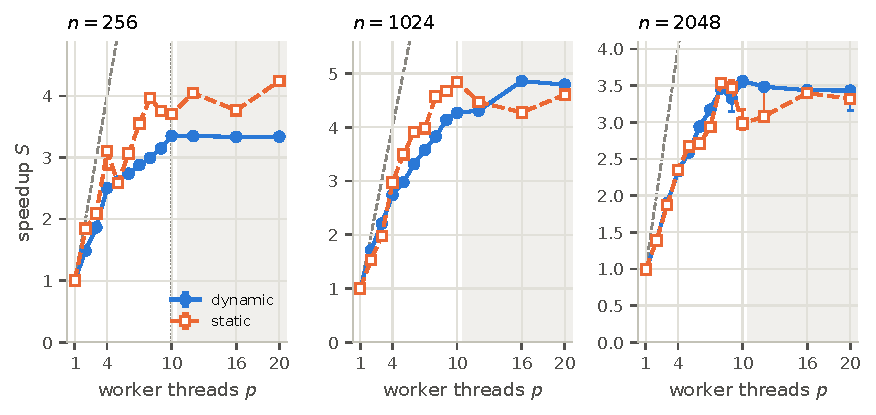
\includegraphics[width=\linewidth]{fig_schedule.pdf}
\caption{Speedup of the static (contiguous bands) and dynamic (row by row)
schedules at $n=256$, 1024 and 2048, with interval bars; dashed: $S=p$.}
\label{fig:schedule}
\end{figure}

\begin{table}[tbp]
\centering
\caption{Speedup of par\_ikj with the dynamic and the static schedule, and busy
cores $U$ of the static runs.}
\label{tab:schedule}
\small
\input{\tabledir/tab_schedule.tex}
\end{table}

\subsection{Oversubscription}

Beyond 10 threads, the dynamic schedule gained nothing at $n=256$ and 512
(within 0.5\% of $p=10$). It lost up to 5.0\% at $n=64$ and at $n=2048$ and
4096. At $n=1024$, 16 and 20 threads were 14 and 12\% faster than 10, with fewer
cycles per multiply-add (0.78 and 0.80 against 0.90) for the same busy cores and
E-core share. At $n=128$, 20 threads were 6\% faster than 10. One process per
configuration and no cache-miss counters cannot tell why.

\subsection{Memory}

At $n\ge2048$ the peak RSS of par\_ikj exceeded that of ikj by 1 to 8\,MiB
for every $p$ (Table~\ref{tab:memory}). Between $p=1$ and 20 it grew from 163
to 169\,MiB at $n=2048$ and from 554 to 559\,MiB at $n=4096$, where it was 1.4
times the $24n^2$ bytes of the three matrices. At small $n$ it grew with $p$.
At $n=64$ it rose from 83\,MiB ($p=1$) to 168\,MiB ($p=20$), against 63\,MiB
for ikj. The heap allocation explains this. At $n=64$, par\_ikj allocated
23.5\,MiB of Java objects over the whole process with one thread and 134.5\,MiB
with 20. Each call builds $p$ task objects and their futures, a process makes
tens of thousands of calls at this size, and the garbage collector ran at most
once per process at $n\le128$, so the garbage stayed in the heap. At $n=1024$,
16 and 20 threads raised the peak RSS by 28 to 31\,MiB without allocating
much more (34.4\,MiB at $p=20$ against 31.7\,MiB at $p=1$); this was not
explained.

\begin{table}[tbp]
\centering
\caption{Peak RSS (MiB) of ikj and par\_ikj (dynamic), Java heap allocated over
the whole process by par\_ikj (MiB), and element storage $24n^2$ (MiB).}
\label{tab:memory}
\small
\input{\tabledir/tab_memory.tex}
\end{table}

\subsection{Vectorisation}

The decoded machine code confirms the vectorisation (Table~\ref{tab:simdcode}).
With SuperWord, the compiled kernels of ikj and of par\_ikj (\texttt{ikjRow},
and the task lambda into which it is inlined) contain 8 \texttt{fmul.2d} and 8
\texttt{fadd.2d} instructions, an inner loop unrolled over 16 elements, two per
instruction. They also contain two scalar multiplies and two scalar adds for the
iterations outside the vector loop. Without SuperWord they contain only scalar
multiplies and adds, 10 of each. No fused multiply-add appears in either.

\begin{table}[tbp]
\centering
\caption{Double-precision floating-point instructions in the final C2-compiled
kernels with SuperWord on and off (\texttt{results/simd}): two-lane vector and
scalar multiplies and adds, fused multiply-adds, and 128-bit loads/stores.}
\label{tab:simdcode}
\footnotesize
\setlength{\tabcolsep}{4pt}
\input{\tabledir/tab_simd_code.tex}
\end{table}

Without SuperWord (Table~\ref{tab:simd}, Fig.~\ref{fig:simd}), the
instructions per multiply-add rose from 3.0--3.5 to 5.8--5.9, by a factor of 1.7
to 2.0. The kernel became 1.46 to 1.51 times slower sequentially, 1.16 to 1.43
times with four threads and 1.32 to 1.40 times with ten. At $n=1024$ and 2048
the gain from vectorisation fell as $p$ grew, from 1.51 and 1.50 at $p=1$ to
1.40 and 1.32 at $p=10$. At $n=512$ the smallest gain was at $p=4$ (1.16). There,
the SuperWord-on run needed 0.80 cycles per multiply-add, 50\% more than the
sequential one.

\begin{table}[tbp]
\centering
\caption{SuperWord on against off: median time per multiplication, the ratio
off/on, and the instructions and cycles per multiply-add (all cores).}
\label{tab:simd}
\small
\input{\tabledir/tab_simd.tex}
\end{table}

\begin{figure}[tbp]
\centering
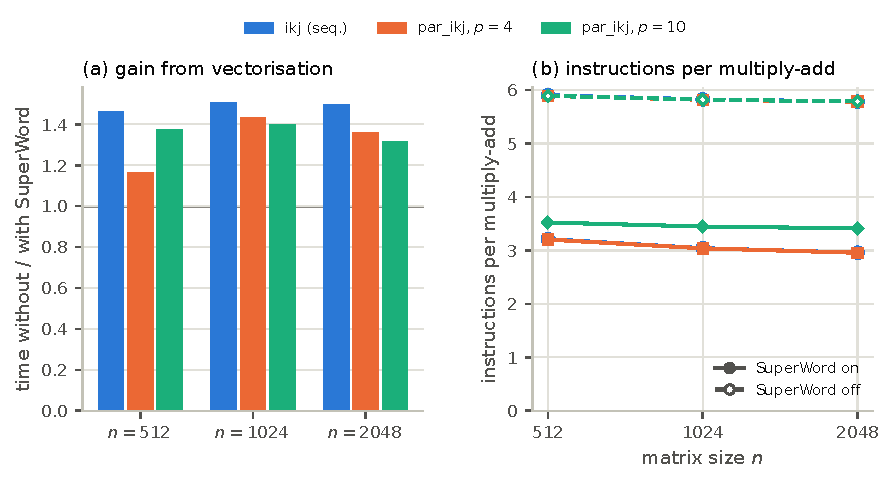
\includegraphics[width=\linewidth]{fig_simd.pdf}
\caption{(a) Time without SuperWord divided by the time with it (above 1:
vectorisation helps). (b) Instructions per multiply-add with SuperWord on
(filled) and off (hollow, dashed); the lines of ikj and of par\_ikj with $p=4$
coincide.}
\label{fig:simd}
\end{figure}

% ===========================================================================
\section{Discussion}
\label{sec:discussion}

\paragraph{Answer to the research question.} On this machine, parallel
execution of the i-k-j kernel helped from $n=128$ on, where one multiplication
lasts 0.3\,ms or more. Four threads, one per P core, gave a speedup of 2.3 to
2.8 at every such size. Beyond four threads, the gain depended on where the
data lived. While $B$ fitted in the caches ($n=256$ to 1024), the E cores
raised the speedup to 3.4 to 4.3 at $p=10$. At $n=4096$, where $B$ streams
from memory, the memory bandwidth held it near 3. At $n=64$ (30\,$\mu$s) waking
the workers cost as much as the work, and parallel execution did not help. The
fastest thread count was 10 or more for $n=256$ to 2048. At $n=4096$ it was 8,
but its speedup of 3.63 is one process in a range of 2.4 to 3.6 for $p\ge4$.
The efficiency never exceeded 0.86 with two or more threads, and it was 0.30 to
0.43 at $p=10$.

\paragraph{H1: identical results.} Supported. Every configuration agreed bit
for bit with every other, in the verification and in all 835 measured
checksums. Each thread computes whole rows with the same operations in the same
order as ikj, and vectorisation does not change the order within an entry of
$C$. Without fused multiply-add~\cite{jep306}, the rounding is the same.

\paragraph{H2: the cost of one thread.} Partly supported. At $n=64$ the
overhead was 24\% (predicted: above 10\%), and from $n=256$ to 1024 it was
within $\pm0.4\%$ (predicted: below 1\% from $n=512$). The cost per call,
7.2\,$\mu$s, was smaller than the predicted tens of microseconds. The prediction
failed at $n=2048$ and 4096, where the one-thread version was 1.9 and 2.1\%
slower. There it ran the same instructions with about 2\% more cycles, which
points to the memory system rather than to the hand-off: the code of
\texttt{ikjRow} is compiled separately from \texttt{ikj}, and the worker is a
different thread from the main one. The session cannot separate these causes.
At $n=4096$, moreover, the two ikj controls differed by 1.2\%, so part of the
gap is variation between processes.

\paragraph{H3: small matrices.} Partly supported. At $n=64$ the speedup stayed
below 2 (at most 1.15). It fell below 1 with one to four threads, not at high
$p$ as predicted: with many threads, the extra workers mostly find no rows left
(2.9 busy cores at $p=10$). This is Amdahl's bound~\cite{amdahl1967} with the
hand-off as the serial part. At $n=128$ the hypothesis failed: the speedup
reached 2.5 to 2.7. A multiplication of 0.3\,ms is long enough for the four P
cores, which took more than 90\% of the rows before the E-core threads joined
in.

\paragraph{H4: P and E cores, static and dynamic.} Partly supported. The first
part held. The gain per added thread was 0.44 to 0.59 up to $p=4$ and 0.03 to
0.26 from 4 to 10 ($n\ge256$). The E-core share was near zero up to $p=4$ and
then followed $(p-4)/p$, and $S(10)$ was well below 10 (at most 4.27). The 4P+6E
capacity line of Fig.~\ref{fig:speedup}, $4+6r=7.6$ at $p=10$, is the speedup
that core types alone would allow if every thread ran as fast as a sequential P
core. The measured 4.0 at $n=512$ is about half of it, because the clock fell
and contention added cycles; the asymmetric chip of Hill and
Marty~\cite{hill2008} is only part of the story.

The second part failed: the static schedule was faster than the dynamic one at
$n=256$ and 1024. Two observations explain why the slowest core did not set the
time. First, the static bands did not stay on the cores where they started. The
E cores did 24 to 38\% of the work, not the 60\% of the rows that six of the
ten bands hold, so macOS moved the remaining bands to the P cores once those
had finished their own. Apple's warning about static
distribution~\cite{appletuning} assumes threads that stay on their cores.
Second, the dynamic schedule paid extra cycles per multiply-add, and the excess
fell roughly as $1/n$, from 0.53 at $n=256$ to 0.22 at 1024 and none at 2048.
The most likely cause is false sharing. Under the dynamic schedule, consecutive
rows go to different threads and are computed at the same time. The rows of $C$
are separate arrays of $8n+16$ bytes, allocated one after another, so the end
of row $i$ and the start of row $i+1$ normally share a 128-byte cache line. Both
threads write that line at each of the $n$ steps of $k$, so it moves between
cores up to $2n$ times per row while the row performs $n^2$ multiply-adds: a
cost per multiply-add proportional to $1/n$. The static bands share only $p-1$
boundaries. The counters do not measure coherence traffic, so this is an
inference. A dynamic schedule with chunks of several rows, or rows padded to
whole cache lines, would test it.

\paragraph{H5: contention for caches and memory.} Supported. The cycles per
multiply-add rose with $p$ for every $n\ge256$. With four threads, all on P
cores and running the same instructions, they were already 1.11 to 1.50 times
the sequential ones. At $p=10$ they were 2.07 and 2.47 times the sequential ones
at $n=2048$ and 4096, against 1.73 to 1.91 at $n=512$ and 1024. The efficiency
at $p=10$ was correspondingly lower at $n\ge2048$ (0.36 and 0.30) than at 512 and
1024 (0.40 and 0.43). No speedup was superlinear. The largest effect appeared
where $B$ fits no cache. At $n=4096$ the kernel requested $B$ at about the
120\,GB/s memory bandwidth of the chip from $p=4$ on, the roofline limit of a
kernel with one multiply-add per 8 bytes~\cite{williams2009}, and the speedup
for 12 to 20 threads, 2.8, equals the ratio of that bandwidth to the
sequential demand to two digits. Speedups above 2.8 at $n=4096$ (up to 3.6) require threads to
share lines of $B$ in the caches, which happens when they work on nearby rows at
the same time. This sharing is not controlled, which may explain why the
speedup at $n=4096$ jumped between 2.4 and 3.6 from one thread count to the next
instead of following $p$.

\paragraph{H6: oversubscription.} Mostly supported. Twelve to twenty threads
cost at most 5\% against ten, within the predicted bound, and gave no further
speedup at five of the seven sizes. The exceptions were $n=1024$ (12 to 14\%
faster with 16 and 20 threads, with fewer cycles per multiply-add) and
$n=128$ (6\% with 20 threads). They are single processes and unexplained.

\paragraph{H7: memory.} Partly refuted. At $n\ge2048$ the peak RSS did not
depend on $p$ beyond 8\,MiB, as predicted. At $n\le128$ it grew by up to
85\,MiB. This is not data shared by the threads but garbage. \texttt{invokeAll}
allocates $p$ task objects and futures on every call, small calls are many, and
with an 8\,GiB heap limit the collector rarely ran. In a long-running service
the same garbage would cost collections instead of resident memory. A reusable
array of tasks would remove it. The 28 to 31\,MiB increase at $n=1024$ with 16
and 20 threads remains unexplained.

\paragraph{H8: vectorisation.} Mostly supported. Without SuperWord the code was
scalar, and the instructions per multiply-add rose by a factor of 1.7 to 2.0,
close to the predicted doubling. The slowdown was largest with one thread (1.46
to 1.51) and smaller at $p=10$, $n=2048$ (1.32), as predicted. More threads
leave less to gain from executing fewer instructions, because the cores spend
more of their cycles waiting for data. The smallest gain, however, was at $p=4$,
$n=512$ (1.16), which the hypothesis did not predict. The SuperWord-on run there
needed 50\% more cycles per multiply-add than the sequential one, which
suggests that the four P cores were already limited by their shared L2 cache.

\paragraph{Limitations.}
\begin{itemize}
  \item \textbf{One machine, one session, one process per configuration.} The
  IQRs describe variation within a process. Between processes, two runs of the
  same configuration differed by up to 7.4\% (ikj, $n=128$) and 15\% (par\_ikj,
  $p=10$, $n=2048$). Comparisons between neighbouring thread counts are
  therefore uncertain by more than their error bars, especially at
  $n\ge2048$ and for $p\ge4$.
  \item \textbf{No affinity.} macOS chose the cores. The measured placement
  (four threads on P cores) is an observation of its scheduler on an idle
  machine, not a controlled factor.
  \item \textbf{Counters, not miss events.} The counters are sums over the whole
  process; cache misses and coherence traffic were not measured. The
  explanations of the schedule result (false sharing) and of the $n=4096$
  limit (memory bandwidth) are inferences from cycles, instructions and the
  requested traffic, not measurements of traffic.
  \item \textbf{JIT variation.} The instructions per multiply-add of par\_ikj
  took different values in different processes of the same size, for example
  2.96 and 3.41 at $n=2048$, so the JIT did not always compile the kernel the
  same way. Single-process comparisons include this variation.
  \item \textbf{Heat.} The fanless machine still throttled at the end of the
  $n=4096$ block (2.59\,GHz in the last control run), despite the cool-down
  pauses. Its effect on the time was small (2.5\%) because that kernel waits for
  memory.
  \item \textbf{Background CPU.} Other processes used a median of 0.06 cores.
  For the session, this figure relies on the per-QoS CPU times instead of
  \texttt{/usr/bin/time} (Section~\ref{sec:protocol}), a substitution checked on
  the pilot and smoke sessions.
\end{itemize}

% ===========================================================================
\section{Conclusions}
\label{sec:conclusions}

For the tested kernel and machine, this study establishes the following:
\begin{enumerate}
  \item A row-parallel i-k-j multiplication on a fixed thread pool is bitwise
  identical to the sequential kernel for any thread count and schedule, with
  or without vectorisation. Rows written by one thread each, and the
  happens-before order of \texttt{invokeAll}, are enough for safe sharing.
  \item Parallel execution helps from $n=128$ on. Four threads give a speedup
  of 2.3 to 2.8, and all ten cores give 3.0 to 4.3 for $n\ge256$, an efficiency
  of 0.30 to 0.43. At $n=64$ it does not help: the hand-off costs about
  7\,$\mu$s per call, and the one-thread version is 24\% slower.
  \item macOS runs four threads on the P cores and every further thread on an E
  core, which retires about half to two thirds of the instructions per second of
  a P core. Together with the clock falling from 4.0 to 3.0--3.8\,GHz as cores
  are added, this explains why ten threads are about four times faster, not ten.
  \item Threads contend for the shared caches and memory: with four threads the
  cycles per multiply-add rise by 11 to 50\%. At $n=4096$ the kernel reaches the
  120\,GB/s memory bandwidth of the chip from about four threads, and its
  speedup stays near 3.
  \item More threads than logical processors cost at most 5\% and gain only in
  isolated cases.
  \item A static assignment of row bands is up to 32\% faster than a row-by-row
  dynamic one at $n=256$ and 1024, despite the heterogeneous cores, most likely
  because the dynamic schedule makes adjacent rows share cache lines between
  threads. The dynamic schedule wins only at $n=2048$, by 8 to 16\% at three
  of the thread counts.
  \item SIMD vectorisation by the JIT (two doubles per instruction) cuts the
  instructions per multiply-add by 40 to 49\% and makes the kernel 1.16 to 1.51
  times faster; it gains less when more threads compete for memory.
  \item Peak memory is independent of $p$ for large matrices. For small ones
  it grows with $p$ because every call allocates task objects.
\end{enumerate}
Four questions remain open. The first is whether false sharing explains the
cost of the dynamic schedule; chunked or padded rows would test it. The second
is why 16 and 20 threads beat 10 at $n=1024$. The third is why the one-thread
version is 2\% slower at $n\ge2048$. The fourth is how much the threads share
$B$ in the caches at $n=4096$. Cache-miss and coherence counters, and several
processes per configuration, would answer them.

% ===========================================================================
\section{References and materials}
\label{sec:materials}

\paragraph{Reproducibility materials.} All code, data and scripts are in the
directory \texttt{assignment3/} of the GitHub repository below, at the tag
\texttt{assignment3-v1.0}:
\begin{center}\repourl\end{center}
Its README gives the exact build and run commands and the software versions.
The materials are:
\begin{itemize}
  \item \texttt{src/}: the Java methods, the process counters, the benchmark
  driver and the JUnit tests; \texttt{pom.xml}: the Maven build.
  \item \texttt{config/bench.json}: the declared protocol, read by every script.
  \item \texttt{scripts/}: input generation (\texttt{gen\_inputs.py}),
  correctness verification (\texttt{verify.py}), the benchmark harness
  (\texttt{run\_benchmarks.py}), the disassembly of the compiled kernels
  (\texttt{simd\_evidence.py}) and the environment snapshot.
  \item \texttt{data/checksums.sha256}: the digests of the inputs, which are
  regenerated in a few seconds instead of being stored.
  \item \texttt{results/correctness.csv}: the outcome of the correctness checks;
  \texttt{results/simd/}: the decoded machine code of the kernels and its
  instruction counts.
  \item \texttt{results/raw/\session/}: every raw sample, warm-ups included
  (\texttt{samples.csv}), one row per process with status, settings, JVM
  activity, peak RSS and background CPU (\texttt{runs.csv}), the environment
  snapshot (\texttt{env.txt}) and the protocol used (\texttt{config.json}).
  \item \texttt{analysis/analyze.py}: the script that produces every table and
  figure in this report from the raw data.
\end{itemize}

\paragraph{Reuse of Assignments 1 and 2.} The baseline kernel, the input
generator and the input files, the correctness tolerance, and the structure of
the benchmark driver, the harness, the verification script and the analysis
script come from Assignment~2 at the tag \texttt{assignment2-v1.0}, which took
the generator, the tolerance and the harness from Assignment~1. The reused
files are adapted copies, and each one names its origin.

\paragraph{Use of generative AI.} Claude Code (Anthropic, model Claude Opus~5.5)
was used as a programming and writing assistant. It helped plan the study, draft
and debug the Java code, tests, scripts and analysis, find the macOS interfaces
for the per-core counters, diagnose the thermal behaviour found in the pilot,
and draft and revise the text of this report. All measurements were produced by
running the code on the author's machine, and every result in
Section~\ref{sec:results} is computed from the committed data by the scripts in
the repository. Each cited source was checked against the original publication
or documentation. The author reviewed the code and the text and is responsible
for the work and its conclusions.

\renewcommand{\refname}{References}
\begin{thebibliography}{99}\raggedright
\small

\bibitem{amdahl1967}
G.~M. Amdahl, ``Validity of the single processor approach to achieving large
scale computing capabilities,'' in \emph{Proc. AFIPS Spring Joint Computer
Conf.}, vol.~30, Atlantic City, NJ, USA, Apr. 1967, pp.~483--485.

\bibitem{hill2008}
M.~D. Hill and M.~R. Marty, ``Amdahl's law in the multicore era,''
\emph{Computer}, vol.~41, no.~7, pp.~33--38, Jul. 2008,
doi: 10.1109/MC.2008.209.

\bibitem{williams2009}
S.~Williams, A.~Waterman, and D.~Patterson, ``Roofline: An insightful visual
performance model for multicore architectures,'' \emph{Commun. ACM}, vol.~52,
no.~4, pp.~65--76, Apr. 2009, doi: 10.1145/1498765.1498785.

\bibitem{hennessy2019}
J.~L. Hennessy and D.~A. Patterson, \emph{Computer Architecture: A Quantitative
Approach}, 6th~ed. Cambridge, MA, USA: Morgan Kaufmann, 2019, ch.~1.

\bibitem{openmp52}
OpenMP Architecture Review Board, ``OpenMP application programming interface,
version 5.2,'' Nov. 2021. [Online]. Available:
\url{https://www.openmp.org/spec-html/5.2/openmp.html}

\bibitem{appletuning}
Apple Inc., ``Tuning your code's performance for Apple silicon,'' Apple
Developer Documentation. Accessed: Oct.~29, 2026. [Online]. Available:
\url{https://developer.apple.com/documentation/apple-silicon/tuning-your-code-s-performance-for-apple-silicon}

\bibitem{jls25}
J.~Gosling, B.~Joy, G.~Steele, G.~Bracha, A.~Buckley, D.~Smith, and G.~Bierman,
\emph{The Java Language Specification, Java SE 25 Edition}. Oracle America,
Inc., 2025, ch.~17. [Online]. Available:
\url{https://docs.oracle.com/javase/specs/jls/se25/html/jls-17.html}

\bibitem{juc25}
Oracle, ``Package java.util.concurrent,'' \emph{Java SE 25 \& JDK 25 API
Specification}, section ``Memory Consistency Properties.'' Accessed: Oct.~29,
2026. [Online]. Available:
\url{https://docs.oracle.com/en/java/javase/25/docs/api/java.base/java/util/concurrent/package-summary.html}

\bibitem{goetz2006}
B.~Goetz, T.~Peierls, J.~Bloch, J.~Bowbeer, D.~Holmes, and D.~Lea, \emph{Java
Concurrency in Practice}. Upper Saddle River, NJ, USA: Addison-Wesley, 2006,
ch.~8.

\bibitem{macsdk}
Apple Inc., \texttt{<sys/resource.h>} (\texttt{struct rusage\_info\_v6}) and
\texttt{<libproc.h>} (\texttt{proc\_pid\_rusage}, \texttt{proc\_pidinfo}), macOS
SDK of the Command Line Tools for Xcode, header files.

\bibitem{larsen2000}
S.~Larsen and S.~Amarasinghe, ``Exploiting superword level parallelism with
multimedia instruction sets,'' in \emph{Proc. ACM SIGPLAN Conf. Programming
Language Design and Implementation (PLDI)}, 2000, pp.~145--156,
doi: 10.1145/349299.349320.

\bibitem{jep306}
J.~Darcy, ``JEP 306: Restore always-strict floating-point semantics,''
OpenJDK, delivered in JDK~17. Accessed: Oct.~29, 2026. [Online]. Available:
\url{https://openjdk.org/jeps/306}

\bibitem{jep454}
M.~Cimadamore, ``JEP 454: Foreign function \& memory API,'' OpenJDK, delivered
in JDK~22. Accessed: Oct.~29, 2026. [Online]. Available:
\url{https://openjdk.org/jeps/454}

\bibitem{georges2007}
A.~Georges, D.~Buytaert, and L.~Eeckhout, ``Statistically rigorous Java
performance evaluation,'' in \emph{Proc. 22nd Annu. ACM SIGPLAN Conf.
Object-Oriented Programming Systems, Languages and Applications (OOPSLA)},
2007, pp.~57--76, doi: 10.1145/1297027.1297033.

\bibitem{higham2002}
N.~J. Higham, \emph{Accuracy and Stability of Numerical Algorithms}, 2nd~ed.
Philadelphia, PA, USA: SIAM, 2002.

\bibitem{applem4}
Apple Inc., ``MacBook Air (15-inch, M4, 2025) -- Tech Specs,'' Apple Support.
Accessed: Nov.~4, 2026. [Online]. Available:
\url{https://support.apple.com/en-us/122210}

\bibitem{harris2020}
C.~R. Harris \emph{et al.}, ``Array programming with NumPy,'' \emph{Nature},
vol.~585, no.~7825, pp.~357--362, Sep. 2020, doi: 10.1038/s41586-020-2649-2.

\end{thebibliography}

\end{document}
